\begin{figure}[h!]
\centering
\begin{subfigure}[t]{0.5\textwidth}
  \captionsetup{justification=centering}
  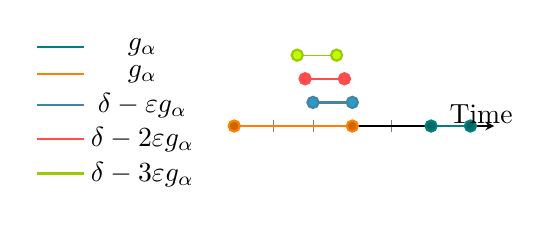
\begin{tikzpicture}
  \begin{axis}[
   axis y line=none,
   y=0.3cm,
   x=1cm,
   xtick={15,15.5,16,...,18},
   restrict y to domain=1:5,
   axis lines=left,
   enlarge x limits=upper,
   cycle list name=exotic,
   scatter/classes={
   o={mark=*,fill=white}
   },
   scatter,
   scatter src=explicit symbolic,
   every axis plot post/.style={mark=*,thick},
   xlabel=Time,
   x label style={at={(axis description cs:0.95,-0.1)},anchor=south},
   xticklabels={,,},
   legend style={
      draw=none,
      at={(-0.1,-1)},
      anchor=south east
  },
  legend image post style={mark=none}
  ]
\addplot table [y expr=1,meta index=1, header=false] {
17.5 c
18 c
};\addlegendentry{$g_{\alpha}$}
\addplot table [y expr=1,meta index=1, header=false] {
15 c
16.5 c
};\addlegendentry{$\backhtxt g_{\alpha}$}
\addplot table [y expr=2,meta index=1, header=false] {
16.5 c
16 c
};\addlegendentry{$\zonep{\delta-\varepsilon}g_{\alpha}$}
\addplot table [y expr=3,meta index=1, header=false] {
16.4 c
15.9 c
};\addlegendentry{$\zonep{\delta-2\varepsilon}g_{\alpha}$}
\addplot table [y expr=4,meta index=1, header=false] {
16.3 c
15.8 c
};\addlegendentry{$\zonep{\delta-3\varepsilon}g_{\alpha}$}
  \end{axis}
  
\end{tikzpicture}
  \caption{Example of an interaction guard $g_{\alpha}$ and its planning intervals}
\end{subfigure}%
\begin{subfigure}[t]{0.5\textwidth}
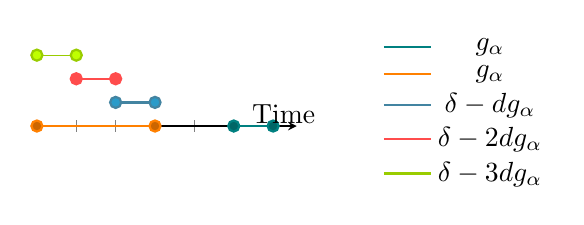
\begin{tikzpicture}
  \begin{axis}[
   axis y line=none,
   y=0.3cm,
   x=1cm,  
   xtick={15,15.5,16,...,18},
   restrict y to domain=1:5,
   axis lines=left,
   enlarge x limits=upper,
   scatter/classes={
   o={mark=*,fill=white}
   },
   scatter,
   cycle list name=exotic,
   scatter src=explicit symbolic,
   every axis plot post/.style={mark=*,thick},
   xlabel=Time,
   x label style={at={(axis description cs:0.95,-0.1)},anchor=south},
   xticklabels={,,},
   legend style={
      draw=none,
      at={(2,-1)},
      anchor=south east
  },
  legend image post style={mark=none}
  ]
\addplot table [y expr=1,meta index=1, header=false] {
17.5 c
18 c
};\addlegendentry{$g_{\alpha}$}
\addplot table [y expr=1,meta index=1, header=false] {
15 c
16.5 c
};\addlegendentry{$\backhtxt g_{\alpha}$}
\addplot table [y expr=2,meta index=1, header=false] {
16.5 c
16 c
};\addlegendentry{$\zonep{\delta-d}g_{\alpha}$}
\addplot table [y expr=3,meta index=1, header=false] {
16 c
15.5 c
};\addlegendentry{$\zonep{\delta-2d}g_{\alpha}$}
\addplot table [y expr=4,meta index=1, header=false] {
15.5 c
15 c
};\addlegendentry{$\zonep{\delta-3d}g_{\alpha}$}
  \end{axis}
  
\end{tikzpicture}
  \caption{Discretized planning intervals for $g_{\alpha}$}
\end{subfigure}
\caption{Discretizing Planning Horizons for Interaction}
\label{fig:disc}
\end{figure}
